\documentclass[12pt,a4paper]{article}
\usepackage[utf8]{inputenc}
\usepackage[T1]{fontenc}
\usepackage{amsmath}
\usepackage{amsfonts}
\usepackage{amssymb}
\usepackage{graphicx}
\usepackage[indonesian]{babel}
\usepackage[left=2.00cm, right=2.00cm, top=2.00cm, bottom=2.00cm]{geometry}
\usepackage{float} 

\title{Tugas 12 - Pengolahan Sinyal Digital\\
	Struktur Jaringan untuk Sistem Infinite Impulse Response (IIR)}

% remove spacing around date:
\usepackage{titling}
\predate{}
\postdate{}
\date{}

\begin{document}
	\maketitle
	\date{}
	\begin{enumerate}
		\item Diketahui sistem linear kausal waktu diskrit yang direpresentasikan dalam persamaan beda berikut ini:
		\[ y(n) - \frac{3}{4}y(n-1) + \frac{1}{8}y(n-2) = x(n) + \frac{1}{3}x(n-1) \]
		Gambarlah grafik aliran sinyalnya untuk mengimplementasikan sistem ini dalam bentuk-bentuk berikut ini:
		\begin{enumerate}
			\item Direct Form I\\
			\textbf{Jawaban:} Pertama adalah implementasikan sisi kanan persamaan beda (zeros) kemudian sisi kiri persamaan (poles). Sehingga direct form I dari persamaan beda tersebut adalah:\\
			\begin{center}
				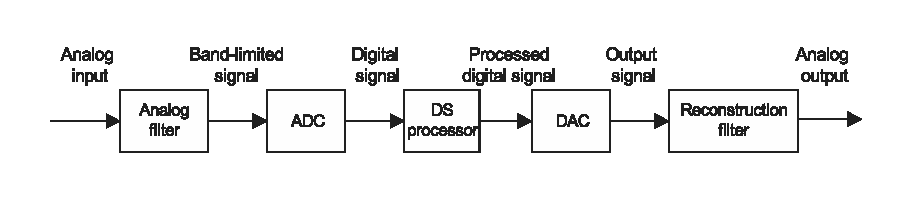
\includegraphics[width=0.7\linewidth]{img/img01}
			\end{center}
			atau yang lebih sederhana
			\begin{center}
				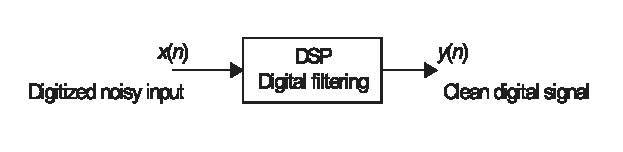
\includegraphics[width=0.5\linewidth]{img/img02}
			\end{center}
			\item Direct Form II
			\textbf{Jawaban:} Implementasikan poles terlebih dahulu kemudian zeros. Sehingga direct form II dari persamaan beda tersebut adalah:\\
			\begin{center}
				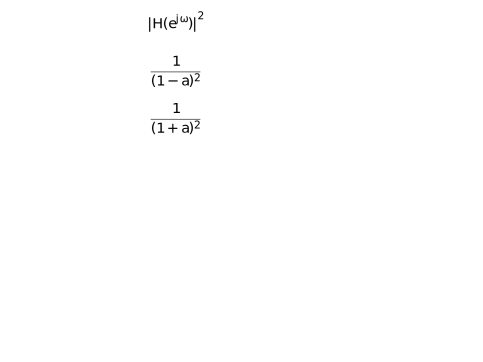
\includegraphics[width=0.7\linewidth]{img/img03}
			\end{center}
			atau bentuk yang lebih sederhana
			\begin{center}
				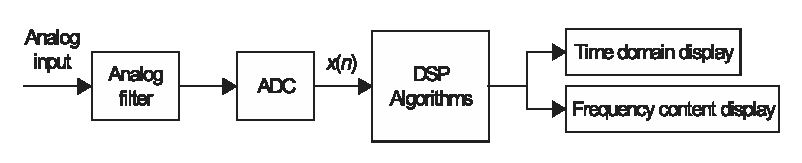
\includegraphics[width=0.5\linewidth]{img/img04}
			\end{center}
			\item Cascade\\
			\textbf{Jawaban:} Pertama adalah memfaktorkan system function kedalam cascade dari 2 sistem orde pertama. Lakukan transformasi Z ke kedua sisi dari persamaan beda:\\
			\[ Y(z)\left[ 1 - \frac{3}{4}z^{-1} + \frac{1}{8}z^{-2} \right] = X(z)\left[ 1 + \frac{1}{3}z^{-1}  \right] \] atau 
			\[ H(z) = \frac{1 + \frac{1}{3}z^{-1}}{1 - \frac{3}{4}z^{-1} + \frac{1}{8}z^{-2}} = \frac{1 + \frac{1}{3}z^{-1}}{(1 - \frac{1}{4}z^{-1})(1 - \frac{1}{2}z^{-1})} \]
			Dalam mengembangkan cascade form, kita sertakan zero dengan pole dan mengatur cascade dalam orde-nya.
			\[ H(z) = \left[ \frac{1 + \frac{1}{3}z^{-1}}{1 - \frac{1}{4}z^{-1}} \right] \left[ \frac{1}{1 - \frac{1}{2}z^{-1}} \right] \]
			Dan dengan menggunakan direct form II untuk subsection pertama, kita dapatkan cascade form-nya
			\begin{center}
				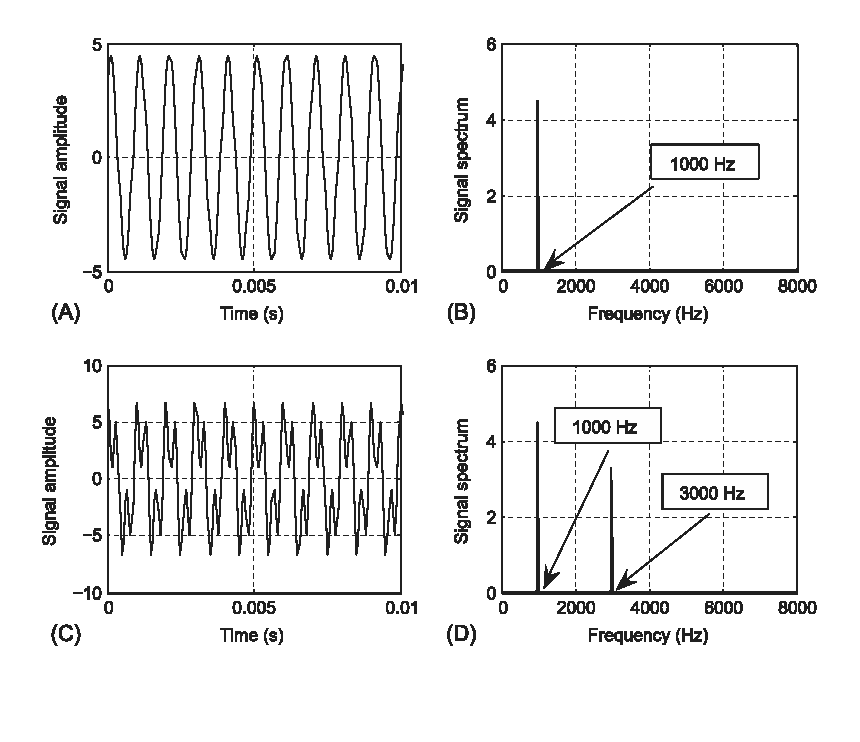
\includegraphics[width=0.5\linewidth]{img/img05}
			\end{center}
			\item Parallel\\
			\textbf{Jawaban:} Parallel form berkaitan dengan melakukan expanding terhadap $ H(z) $ dalam partial fraction expansion. Sehingga:
			\[ H(z) = \frac{10/3}{1 - \frac{1}{2}z^{-1}} + \frac{-7/3}{1 - \frac{1}{4}z^{-1}} \]
			kemudian kita dapatkan
			\begin{center}
				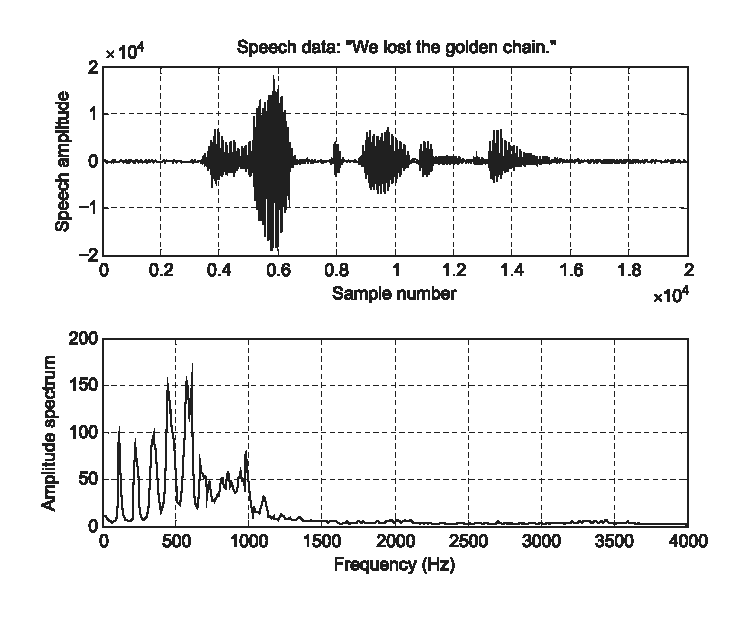
\includegraphics[width=0.5\linewidth]{img/img06}
			\end{center}
		\end{enumerate}
	\end{enumerate}
\end{document}